%--------------------------------------------------------------------------------
\unnumberedChapter{LCS Hardware Module Design}

So far we have covered the general concepts, messages, protocols, and the LCS runtime library. 
We have seen how nodes communicate, how firmware interacts with the runtime, and how the different 
software layers work together.

Now it is time to leave the world of concepts and software for a moment and look at the physical 
side of the system. The LCS runtime and the node firmware need hardware modules to run on. 
Welcome to the next major part of this book: the design and construction of LCS hardware modules.

A hardware module can be viewed as a combination of three fundamental building blocks:

\begin{smallGapItemize}
\item communication
\item controller
\item function block(s)
\end{smallGapItemize}

At the center of every hardware module is the \textbf{controller}. It runs the node firmware and 
provides the processing capabilities needed for the specific module. There are many controller 
families and development environments available today. Selecting the right controller is therefore 
an important design decision.

A good controller needs sufficient processing power, enough memory, and a powerful development 
environment. Easy software loading, debugging capabilities, and a convenient console interface are 
also very valuable during development and operation.

The second building block is \textbf{communication}. Every LCS module needs at least one communication 
interface to participate in the LCS network. The primary communication method used by LCS is the CAN 
bus. The communication hardware provides the physical interface while the software layer implements 
the LCS messaging model described earlier in this book.

Finally, the \textbf{function blocks} implement the module-specific capabilities. A block controller 
needs power electronics and track monitoring. A handheld needs user input devices and a display. 
A sensor module needs input circuitry, while an actuator module may need drivers for LEDs, signals, 
or turnouts.

The idea behind the hardware design is similar to the software design introduced earlier. Instead of 
creating every module as a completely independent design, we define reusable building blocks that can 
be combined to create different hardware modules.

This part of the book introduces these hardware building blocks one at a time. The goal is to 
understand how each component works and how it can be combined with the others. Later chapters will 
then use these building blocks to create complete modules such as the base station, block controller, 
and other LCS devices.


%-------------------------------------------------------------------------------------------------------
\unnumberedSection{Selecting the controller}

The first hardware designs described in this book started with the AtMega controller family together 
with the Arduino development environment. Controllers such as the Arduino UNO, Arduino NANO, and 
Arduino MEGA have been widely used in hobby projects for many years. They are inexpensive, well 
documented, and supported by a large community.

For the first experiments, these controllers were a natural choice. However, as the LCS software 
architecture evolved, the requirements increased. The LCS runtime library provides many services 
that require additional memory and processing capability. Non-volatile storage management, event 
handling, message processing, and the ability to run more complex node firmware all place higher 
demands on the controller platform.

The AtMega family is still an excellent choice for many embedded applications. However, for the LCS 
system a more capable platform provides more room for future development.

The Raspberry Pi Pico joined the available controller platforms at exactly the right time. It offers 
a significant increase in capability while remaining inexpensive and easy to use. The PICO is based 
on a dual-core processor running at up to 200\,MHz. It provides 264\,Kbytes of RAM, 16\,Mbytes of 
flash memory, and a rich set of peripheral interfaces including UART, SPI, and I2C.

However, the most interesting feature for the LCS project is the programmable I/O system, commonly 
called PIO. These programmable state machines allow dedicated hardware-like functions to be 
implemented in software. This opens interesting possibilities for communication protocols and timing 
critical tasks.

One example is the CAN bus implementation used by LCS. Instead of requiring a dedicated CAN 
controller chip, the \textbf{can2040} library uses the PIO state machines of the PICO to implement 
the CAN protocol. The result is a very compact solution: only the CAN transceiver hardware is 
required in addition to the controller.

This is one of those small but powerful design features that makes the PICO particularly attractive 
for this project.

The dual-core architecture is also a good match for the LCS requirements. One processor core can 
handle the application firmware and runtime activities, while the second core is dedicated to the 
CAN communication processing.

The firmware development environment has also evolved together with the hardware. The current LCS 
software is developed using Visual Studio Code together with CMake-based build management. This 
provides a consistent environment for managing libraries and applications and ensures that the 
different software components remain synchronized as the project grows.

Although other capable controllers will certainly appear in the future, a project also needs a stable 
foundation. Constantly changing controllers makes completing a system difficult. For LCS, the 
Raspberry Pi Pico is the selected controller platform because its capabilities match the requirements 
very well and provide sufficient resources for future expansion.

Nevertheless, the LCS software architecture is designed to be as independent from a specific 
controller as possible. The controller-specific parts are isolated in the Controller Dependent Code 
layer introduced in the firmware section. This keeps the possibility open to use other controller 
families in the future.


%-------------------------------------------------------------------------------------------------------
\unnumberedSection{The Controller Platform}

The following table summarizes the controller capabilities typically required for an LCS hardware 
module. Although the examples are based on the Raspberry Pi Pico, the requirements are generally 
applicable to other controller platforms as well.

\begin{longtable}{@{}p{0.25\linewidth}p{0.6\linewidth}@{}}
    \caption{Controller Attributes} \\
    \toprule
    \textbf{Attributes} & \textbf{Notes} \\
    \midrule
    \endfirsthead
    \toprule
    \textbf{Attributes} & \textbf{Notes} \\
    \midrule
    \endhead
    \midrule
    \multicolumn{2}{r}{\textit{Continued on next page}} \\
    \midrule
    \endfoot
    \bottomrule
    \endlastfoot
    \textbf{Processor} & For a typical module, the PICO offers plenty in terms of CPU power. Since we use a software implementation for the CAN bus, running the software in one core and the CAN bus state machine in the other will well match what the PICO offers. \\
    \midrule
    \textbf{Memory} & Memory depends on the size requirements of the node, port and event maps and the node-specific firmware data demands. A simple module would perhaps get by with 2Kb, a base station could easily use 32Kb or even more. \\
    \midrule
    \textbf{Program Memory} & The LCS library already uses round about 64Kb of code storage. A simple module would get by with 32Kb, a base station could easily use 128Kb and more. \\
    \midrule
    \textbf{External NVM} & Additional NVM storage is allocated in a separate EEPROM or FRAM. The capacity is highly dependent on the module use case. External NVM components typically also require the SPI or I2C interface. Most external EEPROM chips have write cycles of more than a million. At a minimum, a chip size of 32Kb is recommended. The PICO does not offer an internal EEPROM, so an external NVM is always required. \\
    \midrule
    \textbf{Digital channels} & The bulk of control lines is digital and used heavily. For some hardware modules, a subset of the digital pins should also be PWM capable. \\
    \midrule
    \textbf{Analog channels} & Analog input is typically used for the power module for analog voltage measurements. Otherwise, it is perhaps optional. The PICO allows for only three inputs. If more are desired, an external multiplexer needs to be implemented. \\
    \midrule
    \textbf{I2C} & The I2C interface comes in very handy to connect a large variety of chips. Communication to the external NVM and also to chips that implement functions such as a servo controller will require this bus. \\
    \midrule
    \textbf{Serial I/O} & The serial I/O is used in some hardware modules for implementation of RailCom detectors. The PICO features two hardware UARTS and the option to implement more in software using the PIO state machines. \\
    \midrule
    \textbf{Console I/O} & Serial I/O is used for console I/O. Rather than using dedicated I/O pins and a UART block in the controller, the PICO serial I/O will be implemented via the USB connector. \\
    \midrule
    \textbf{Programmable IO} & Some controllers, for example the PICO, offer a programmable IO interface or programmable logic on the controller chip. This is a very handy feature for implementing complex signal generation. \\
    \midrule
    \textbf{LEDs, Buttons and Dip Switches} & A hardware module could make use of LEDs to indicate readiness and activity, as well as providing a set of switches to configure a hardware option. Not really required but certainly useful. \\
    \midrule
    \textbf{WLAN} & WLAN is optional, but becoming really popular. There is a PICO version with WLAN capability integrated. \\
\end{longtable}

%-------------------------------------------------------------------------------------------------------
\unnumberedSection{Communication and the CAN Bus}

Communication is one of the fundamental building blocks of every LCS hardware module. 
The LCS architecture uses the CAN bus as the communication backbone between nodes.

From a hardware perspective, controllers usually provide one of two approaches. Some controllers 
include a dedicated CAN controller as an internal hardware block. Others require an external CAN 
controller chip, such as the MCP2515, connected through a serial interface.

The Raspberry Pi Pico takes an interesting alternative approach. Its programmable I/O state machines 
allow communication protocols to be implemented directly in hardware-assisted software. The 
\textbf{can2040} library uses this capability to implement a complete CAN controller using the PIO 
state machines.

This is a very elegant solution. The hardware module only requires the physical CAN transceiver 
connected to the controller. No additional CAN controller chip is needed. The PIO state machine takes 
care of the timing-critical CAN protocol processing while the main firmware can focus on the LCS 
application.

The dual-core architecture of the PICO fits this design particularly well. One core is dedicated to 
the communication processing, while the other core executes the runtime and application firmware.

The use of PIO state machines will appear several times throughout the hardware design. They are not 
only useful for communication. They can also replace dedicated logic components for timing-critical 
tasks.

For example, the block controller design later in this book uses PIO state machines to assist with 
DCC signal processing, H-bridge control timing, cutout period handling, and RailCom datagram 
detection. Instead of adding several dedicated logic components, these functions can be implemented 
close to the controller itself.

%-------------------------------------------------------------------------------------------------------
\unnumberedSection{Hardware Module Schematics}

Hardware modules are described to a large extent through their schematics. The schematics shown 
throughout this book were created using the \textbf{EasyEDA} design environment. EasyEDA provides a 
complete workflow from schematic capture to PCB layout and manufacturing.

The hardware design follows the same building block philosophy used throughout the LCS software. 
Instead of drawing every module as one large schematic, functional blocks are created separately and 
combined when building a complete hardware module.

Each building block contains clearly defined connection points. These connection points are named 
using a unique network identifier. When two blocks use the same network name, the signals are 
connected when the blocks are combined into a complete schematic.

For example, the network name \texttt{VCC-3V3} always refers to the 3.3V supply line. Any building 
block containing this connection will automatically connect to the same power supply when used in a 
module design.

This approach makes the schematics easier to understand and reuse. A CAN interface block, a power 
supply block, or an I2C interface block can be reused in different hardware modules without 
redrawing the complete circuit.

The building blocks shown in this book should be understood as reference implementations. They 
describe how a function can be implemented and explain the assumptions made by the LCS software.

The runtime library has intentionally been designed with hardware independence in mind. However, the 
final implementation always requires adaptation to the selected controller, including timers, 
communication interfaces, GPIO assignments, and other hardware resources.

Throughout the hardware chapters, comments will identify which parts are generic and which parts are 
specific to the Raspberry Pi Pico implementation.


%-------------------------------------------------------------------------------------------------------
\unnumberedSection{General Board Layout}

Every LCS node requires a controller running the node firmware. While different nodes will require 
different hardware functions, they all share a common foundation:

\begin{smallGapItemize}
\item a controller
\item a power supply connection
\item an LCS bus interface
\item optional external non-volatile storage
\item node-specific function hardware
\end{smallGapItemize}

One possible approach would be to design every hardware module as a completely independent board. 
For a small number of modules this is a reasonable solution. However, many modules would then 
contain the same controller, communication, and power supply circuitry repeatedly.

The approach chosen for LCS is based on reusable hardware building blocks. A common controller board 
provides the basic platform for a node. Extension boards then add the specific hardware functions 
required by a particular module.

This is similar to the concept of expansion boards used in many controller ecosystems. However, the 
LCS design extends this idea further. Extension boards can either be directly connected to the 
controller board or several boards can be combined using a backplane.

This provides flexibility. A simple sensor module may only require the controller board and a small 
extension board. A complex module such as the base station or block controller can combine several 
functions into one larger hardware design.

Before looking at individual modules, we first define the physical layout and connectors used by all 
boards.

\begin{figure}[ht]
	\centering
	\begin{tikzpicture}[scale=0.9, transform shape]

    	% \draw[help lines, gray!50, dashed] (0,0) grid (16,8);

    	\node at (8,4) {
        	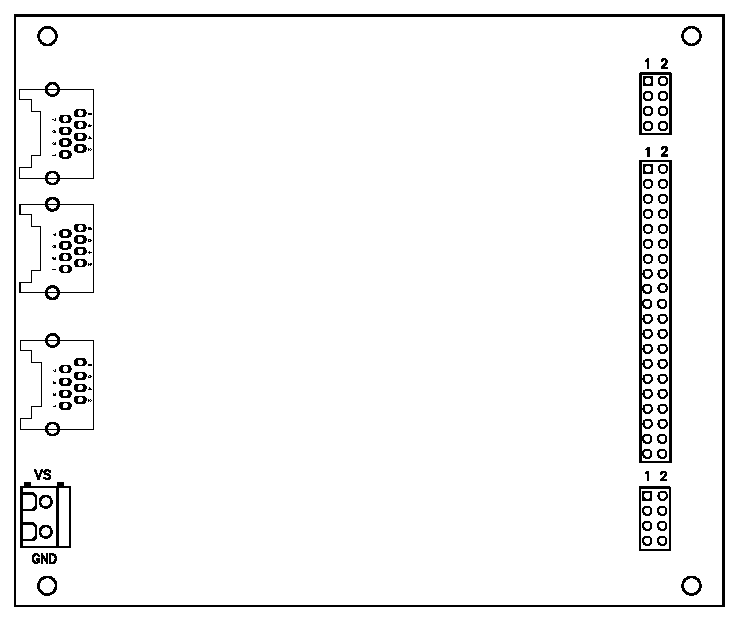
\includegraphics[page=1, scale=0.7]
				{./part-hardware/chapter-hardware-module-design/LCS-FP-MAIN-10X12.pdf}
    	};
    	
    	\draw[decorate, decoration={brace, amplitude=6pt}] (3.25,4.25) -- (3.25,6.5);
    	\node at ( 1, 5.4 ) {LCS Bus};
    	
    	\draw[->] (3, 3.25) -- (3.5, 3.25);
    	\node at ( 1, 3.25 ) {I2C Bus};

		\draw[->] (3, 1.5) -- (3.5, 1.5);
    	\node at ( 1, 1.5 ) {Power};
    	    	
    	\draw[decorate, decoration={brace, mirror, amplitude=6pt}] (13,1) -- (13,6.5);
    	\node [rotate=90] at ( 14, 4 ) {Extension Connector };

	\end{tikzpicture}
\end{figure}
\FloatBarrier

All boards follow a common form factor. The standard widths and lengths allow boards to be combined 
mechanically while keeping the connector positions consistent.

The main controller board contains the external connections on the left side:

\begin{smallGapItemize}
\item LCS bus connection
\item external I2C bus
\item power input
\end{smallGapItemize}

The extension connector is located on the right side. This connector is optional and allows 
additional functionality to be attached.

To simplify schematic creation and ensure mechanical compatibility, EasyEDA symbols and PCB 
footprints are provided for the supported board dimensions and connector locations.


%-------------------------------------------------------------------------------------------------------
\unnumberedSection{LCS Bus Connector}

Every hardware module needs access to the LCS bus. Some smaller modules may also receive their power 
from the bus, while larger modules such as boosters or block controllers use a separate power supply.

The physical connection uses an RJ45 connector. Although commonly associated with Ethernet, the RJ45 
connector provides a convenient and inexpensive multi-wire connection for the different signals 
required by LCS.

The signals on the LCS bus can be grouped into several categories.

The first group is the CAN differential pair. These two signals form the communication backbone of 
the layout control system.

The second group provides power. The \texttt{PWR} line is intended for modules with low power 
requirements. Modules with higher power consumption should use their own power input.

The third group contains the DCC signal lines. These signals carry an exact copy of the generated 
track signal and are primarily intended for distribution from the base station to boosters or 
analysis modules.

Finally, the \texttt{STOP} line provides a simple emergency mechanism. It is implemented as a shared 
active-low line that allows any connected device to request a layout stop condition.

\begin{longtable}{@{}|l|l|p{0.6\linewidth}|@{}}
    %\caption{LCS Bus Connector Pins}
    \toprule
    \textbf{Pin} & \textbf{Name} & \textbf{Purpose} \\
    \midrule
    \endfirsthead
    \toprule
    \textbf{Pin} & \textbf{Name} & \textbf{Purpose} \\
    \midrule
    \endhead
    \midrule
    \multicolumn{2}{r}{\textit{Continued on next page}} \\
    \midrule
    \endfoot
    \bottomrule
    \endlastfoot
    1 & DCC-Sig-1 & The DCC signal labelled "+" \\
    \midrule
    2 & DCC-Sig-2 & The DCC signal labelled "-" \\
    \midrule
    3 & STOP & shared line for an active low signal. \\
    \midrule
    4 & GND & common ground. \\
    \midrule
    5 & GND & common ground. \\
    \midrule
    6 & PWR & The bus supplied 12V power line. This line is intended for devices with very little power consumption to get their power from. Module with high power consumption should connect to its own power supply line. \\
    \midrule
    7 & CAN-L &  Line L of the differential CAN bus signal. \\
    \midrule
    8 & CAN-H &  Line H of the differential CAN bus signal. \\
\end{longtable}
\FloatBarrier

%-------------------------------------------------------------------------------------------------------
\unnumberedSection{I2C Bus Connector}

In addition to the LCS bus, the controller board exposes an external I2C interface. The I2C bus is 
used primarily for communication with extension boards and additional peripheral components.

I2C is a good match for the LCS hardware concept. Many integrated circuits are available with an 
I2C interface, including memory devices, sensor components, display controllers, and dedicated 
interface chips. Using I2C allows additional functionality to be added without consuming many 
controller GPIO pins.

The external I2C connector is available both on the controller board and on extension boards. 
Extension boards typically use this interface as their primary communication channel with the 
controller board.

\begin{longtable}{@{}|l|l|p{0.6\linewidth}|@{}}
    %\caption{I2C Bus Connector Pins}
    \toprule
    \textbf{Pin} & \textbf{Name} & \textbf{Purpose} \\
    \midrule
    \endfirsthead
    \toprule
    \textbf{Pin} & \textbf{Name} & \textbf{Purpose} \\
    \midrule
    \endhead
    \midrule
    \multicolumn{2}{r}{\textit{Continued on next page}} \\
    \midrule
    \endfoot
    \bottomrule
    \endlastfoot
    1 & VCC & The power line. \\
    \midrule
    2 & VCC & The power line. \\
    \midrule
    3 &  & not used. \\
    \midrule
    4 & SCL & The I2C SCL line. \\
    \midrule
    5 & SDA & The I2C SDA line. \\
    \midrule
    6 &  & not used. \\
    \midrule
    7 & GND & The power line. 5V. \\
    \midrule
    8 & GND & The power line. 5V. \\  
\end{longtable}
\FloatBarrier

The I2C bus is not intended to replace the LCS CAN bus. The two interfaces serve different purposes. 
The CAN bus provides the communication backbone between independent LCS nodes, while the I2C bus is 
used locally between components that belong to the same hardware module.

%-------------------------------------------------------------------------------------------------------
\unnumberedSection{LCS Node Extension Board Connector}

To make extension boards interchangeable, a standardized connector is defined between the controller 
board and extension boards.

An extension board provides a male connector on its left side, while the controller board provides 
the matching female connector on its right side. This allows extension boards to be placed directly 
next to the controller board.

The same connector concept also supports a backplane arrangement. In this case, several extension 
boards can be connected next to the controller board instead of stacking directly.

The concept is similar to the shield ecosystem used by platforms such as Arduino or Raspberry Pi. 
However, the LCS approach is designed specifically for layout control modules and allows both direct 
connection and backplane-style arrangements.

The primary communication method between controller and extension boards is the I2C bus. In fact, 
most current extension boards only require the I2C interface and power supply.

Nevertheless, the connector provides additional controller resources. This leaves room for more 
complex extension boards that require direct access to controller capabilities such as digital I/O, 
analog inputs, PWM outputs, or serial interfaces.

The Raspberry Pi Pico provides a very flexible pin assignment system. Many peripheral functions can 
be mapped to different GPIO pins. The extension connector therefore exposes a carefully selected set 
of signals that allow the capabilities of the controller to be used by extension boards.

% ---------------------------------------------------------------------------
% Insert extension connector figure here
% ---------------------------------------------------------------------------

\begin{longtable}{@{}|p{0.1\linewidth}|p{0.1\linewidth}|p{0.1\linewidth}|p{0.1\linewidth}|p{0.4\linewidth}|@{}}
    \caption{Extension Connector} \\
    \toprule
    \textbf{Pin} & \textbf{Name} & \textbf{Pin} & \textbf{Name} & \textbf{Purpose} \\
    \midrule
    \endfirsthead
    \toprule
    \textbf{Pin} & \textbf{Name} & \textbf{Pin} & \textbf{Name} & \textbf{Purpose} \\
    \midrule
    \endhead
    \midrule
    \multicolumn{2}{r}{\textit{Continued on next page}} \\
    \midrule
    \endfoot
    \bottomrule
    \endlastfoot
    1 & \textbf{O-0-1} & 2 & \textbf{O-0-2} & Track 1 "+"\\
    \midrule
    3 & \textbf{O-1-1} & 4 & \textbf{O-1-2} & Track 1 "-"\\
    \midrule
    5 & \textbf{O-2-1} & 6 & \textbf{O-2-2} & Track 2 "+"\\
    \midrule
    7 & \textbf{O-3-1} & 8 & \textbf{O-3-2} & Track 2 "-"\\
    \midrule
    \midrule
    \midrule
    1 & \textbf{GND} & 2 & \textbf{GND} & Ground \\
    \midrule
    3 & \textbf{DCC-1} & 4 & \textbf{DCC-2} & The DCC "+" and "-" signal as generated by the DCC Signal Generator. "+" refers to DCC-1. These pins are typically driven by the base station generating the layout DCC signal.\\
    \midrule
    5 & \textbf{GND} & 6 & \textbf{GND} & Common ground pins. \\
    \midrule
    7 & \textbf{ADC-0} & 8 & \textbf{ADC-1} & Analog input pins. The input is not protected. The analog voltage range is 0 to VCC. \\
    \midrule
    9 & \textbf{GND} & 10 & \textbf{GND} & Common ground pins. \\
    \midrule
    11 & \textbf{DIO-0} & 12 & \textbf{DIO-1} & Plain digital Pins, input or output. The pins are protected. \\
    \midrule
    13 & \textbf{DIO-2} & 14 & \textbf{DIO-3} & Plain digital Pins, input or output. The pins are protected. \\
    \midrule
    15 & \textbf{DIO-4} & 16 & \textbf{DIO-5} & Plain digital Pins, input or output. The pins are protected. \\
    \midrule
    17 & \textbf{DIO-6} & 18 & \textbf{DIO-7} & Plain digital Pins, input or output. The pins are protected. \\
    \midrule
    19 & \textbf{DIO-8} & 20 & \textbf{DIO-9} & Plain digital Pins, input or output. The pins are protected. \\
    \midrule
    21 & \textbf{DIO-10} & 22 & \textbf{DIO-11} & Plain digital Pins, input or output. The pins are protected. \\
    \midrule
    23 & \textbf{GND} & 24 & \textbf{GND} & Common ground pins. \\
    \midrule
    25 & \textbf{SCL} & 26 & \textbf{SDA} & I2C extension bus channel.  The lines are protected with a serial resistor and there is a pull-up resistor to VCC. \\
    \midrule
    27 & \textbf{RST} & 28 & \textbf{EXT} & RST is reset line. Active Low. EXT is the external interrupt line which be raised from an extension board. Active low. \\
    \midrule
    29 & \textbf{GND} & 30 & \textbf{GND} & Common ground pins. \\
    \midrule
    31 & \textbf{VCC} & 32 & \textbf{VCC} & VCC 5V supply to extension boards. \\
    \midrule
    33 & \textbf{GND} & 34 & \textbf{GND} & Common ground pins. \\
    \midrule
    35 & \textbf{VS} & 36 & \textbf{VS} & Board Input voltage forward. These  connector pins are primarily used by extension boards that need the high power input. Examples  are H-Bridges on such a board or boards that have their power supply circuitry. \\
    \midrule
    37 & \textbf{VS} & 38 & \textbf{VS} & Board Input voltage forward. \\
    \midrule
    39 & \textbf{GND} & 40 & \textbf{GND} & Common ground pins. \\
    \midrule
    \midrule
    \midrule
    1 & \textbf{O-4-1} & 2 & \textbf{O-4-2} & Track 3 "+" \\
    \midrule
    3 & \textbf{O-5-1} & 4 & \textbf{O-5-2} & Track 3 "-"\\
    \midrule
    5 & \textbf{O-6-1} & 6 & \textbf{O-6-2} & Track 4 "+"\\
    \midrule
    7 & \textbf{O-7-1} & 8 & \textbf{O-7-2} & Track 4 "-"\\
    \midrule
\end{longtable}  


The extension connector consists of three physical connector groups.

The central connector provides the general-purpose interface between controller and extension 
boards. It contains power, communication signals, and GPIO connections.

Two additional connectors provide track-related signals. These connectors are primarily intended for 
modules such as the base station and block controller where several track outputs need to be 
connected to extension hardware.



%-------------------------------------------------------------------------------------------------------
\unnumberedSection{Controller, Extension and Socket Boards}

The combination of controller and extension boards forms a complete LCS node. The controller board 
provides the common infrastructure, while extension boards add the hardware functions required by a 
specific application.

There are two basic ways of using this concept.

The first option is a direct connection. An extension board is plugged directly into the controller 
board connector. This is suitable when the additional hardware belongs physically close to the 
controller.

The second option uses a backplane arrangement. Several extension boards can be placed next to each 
other together with the controller board. Electrically, the concept remains identical; only the 
mechanical arrangement changes.

\begin{figure}[ht]
    \centering
    \begin{tikzpicture}[scale=1, transform shape]
        \useasboundingbox (0,0) rectangle (15,10.5);
        % \draw[help lines, gray!50, dashed] (0,0) grid(15,10.5);
        
        \node at (3.5, 6.5) {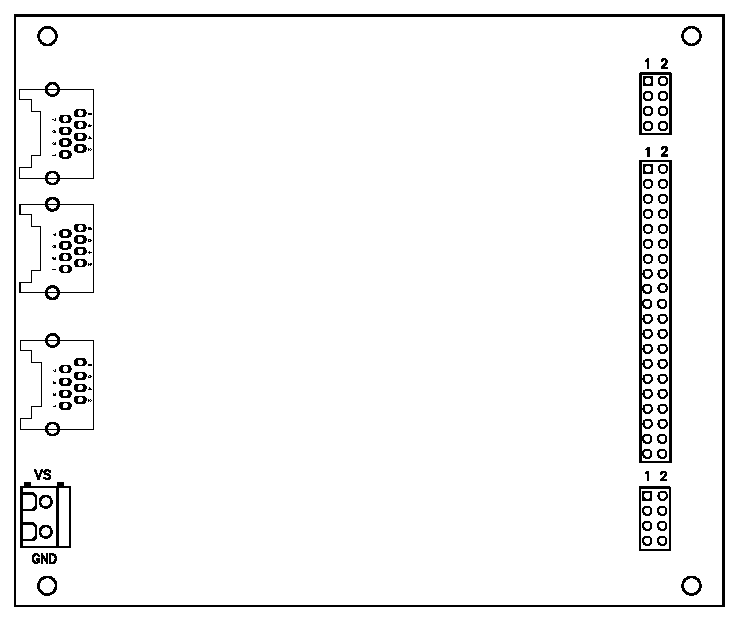
\includegraphics[page=1, scale=0.5]
				{./part-hardware/chapter-hardware-module-design/LCS-FP-MAIN-10X12.pdf}};
				
		\node at (12, 7) {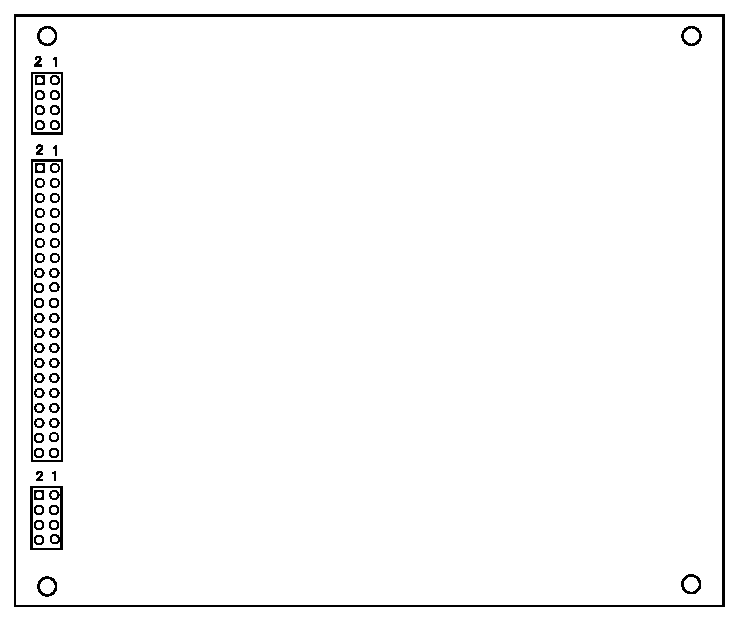
\includegraphics[page=1, scale=0.5]
				{./part-hardware/chapter-hardware-module-design/LCS-FP-EXT-10X12.pdf}};

        \node at (11.5, 6.5) {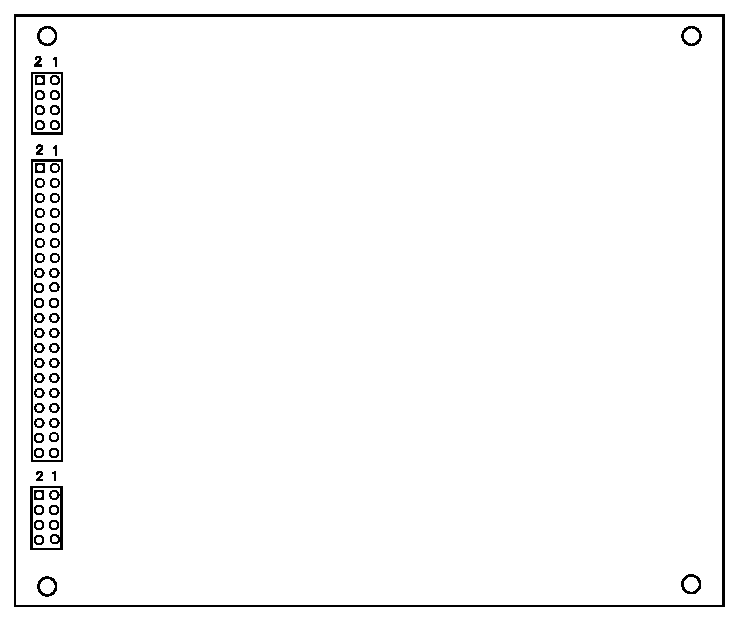
\includegraphics[page=1, scale=0.5]
				{./part-hardware/chapter-hardware-module-design/LCS-FP-EXT-10X12.pdf}};

        \node at (3, 10) {\textbf{Main Controller Board}};
        \node at (11, 10) {\textbf{Extension Board(s)}};
        \node at (13.5, 1.5) {\textbf{Socket Boards}};
        
        \draw[line width=1mm, gray!40, ->] (5,6.5) -- (10,6.5);
        
        \node at (3.5, 1.5) {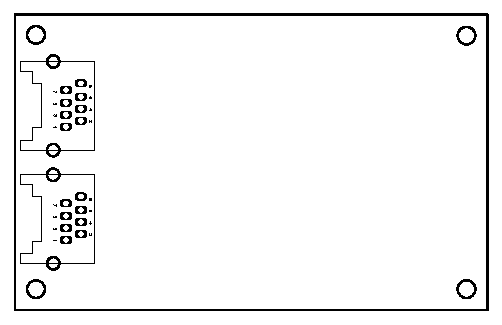
\includegraphics[page=1, scale=0.35,  angle=270]
				{./part-hardware/chapter-hardware-module-design/LCS-FP-SOCKET-5X8.pdf}};
				
		\node at (6.5, 1.5) {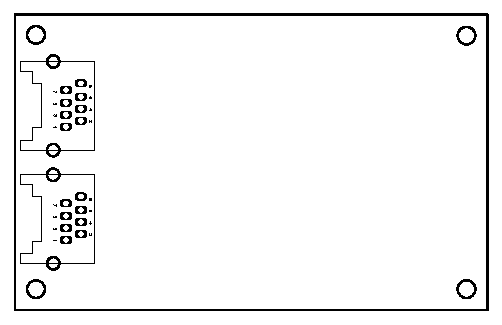
\includegraphics[page=1, scale=0.35,  angle=270]
				{./part-hardware/chapter-hardware-module-design/LCS-FP-SOCKET-5X8.pdf}};
				
		\node at (10.5, 1.5) {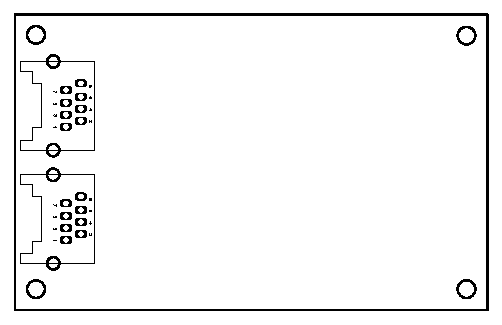
\includegraphics[page=1, scale=0.35,  angle=270]
				{./part-hardware/chapter-hardware-module-design/LCS-FP-SOCKET-5X8.pdf}};
				
		\draw[line width=0.5mm, gray!40, <->] (0.5,5.85) -- (0.25,5.85) -- (0.25, 3.25) -- (3.2, 3.25) -- (3.2, 3);
    	\draw[line width=0.5mm, gray!40, <->] (3.75,3) -- (3.75,3.25) -- (6.2,3.25) -- (6.2,3);
    	\draw[line width=0.5mm, gray!40, <->] (6.75,3) -- (6.75,3.25) -- (10.2,3.25) -- (10.2,3);
    	
    \end{tikzpicture}
    \caption{Connecting boards}
\end{figure}
\FloatBarrier


The advantage of this approach becomes visible when looking at the range of possible LCS modules.

A small sensor node may consist of only a controller board and a small extension board. A signal 
module may add LED drivers and output circuitry. A base station or block controller may combine the 
controller board with several specialized extension boards containing powerful hardware functions.

The same basic controller platform can therefore serve many different purposes.


%-------------------------------------------------------------------------------------------------------
\unnumberedSection{Socket Extension Board}

While extension boards add functionality to the controller board, some functions are better located 
close to the physical element they control.

For example, a turnout or signal may be located several meters away from the main controller. Running 
many individual wires back to a central extension board would not be practical.

For these cases, small socket extension boards are used.

Socket boards are connected to an extension board through the I2C bus and receive their power through 
the same connection. They provide a local interface close to the controlled element.

Typical examples are:

\begin{smallGapItemize}
\item a turnout driver located close to a turnout
\item a signal driver located close to a signal mast
\item a small sensor interface located close to a detector
\end{smallGapItemize}

The extension board provides the more powerful local hardware resources, while socket boards provide 
a simple way to distribute the physical connections around the layout.

The separation also keeps the wiring of the layout manageable. Instead of bringing every individual 
signal wire back to a central location, small local modules can be placed where they are needed.

Since only a limited number of extension boards are normally connected to one controller, the signal 
line lengths remain reasonable. For more compact arrangements, extension boards with only the right 
side connector can be inserted into a backplane board together with the controller board.

The electrical concept remains unchanged. Only the mechanical arrangement is different.

\begin{figure}[ht]
    \centering
    \begin{tikzpicture}[scale=1, transform shape]
        \useasboundingbox (0,0) rectangle (15,5);
        \draw[help lines, gray!50, dashed] (0,0) grid(15,5);
        
        \node at (12.5, 2) {\textbf{Socket Board}};
        
        \node at (1.5, 4) {\textbf{I2C Bus}};

        \draw[line width=0.5mm, gray!30, <-] (1,0) -- (1,1.5) -- (4, 1.5);
        \draw[line width=0.5mm, gray!30, ->] (1, 3.5) -- ( 1, 2.5) -- (4,2.5);
        
        \node at (7.5, 2) {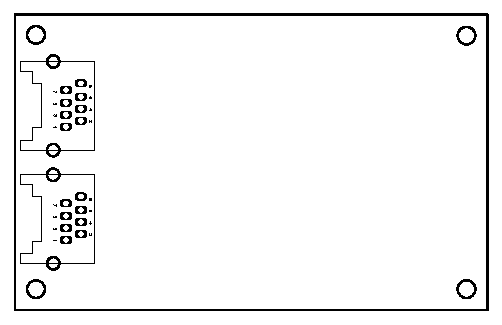
\includegraphics[page=1, scale=0.7]
				{./part-hardware/chapter-hardware-module-design/LCS-FP-SOCKET-5X8.pdf}};  	
    	
    \end{tikzpicture}
\end{figure}
\FloatBarrier

%-------------------------------------------------------------------------------------------------------
\unnumberedSection{Summary}

This chapter introduced the basic hardware design philosophy behind LCS modules.

A hardware module is built from three fundamental parts: communication, controller, and function 
blocks. The controller provides the processing platform, the communication interface connects the 
module to the LCS network, and the function blocks implement the actual purpose of the module.

A central idea is the reuse of common building blocks. Instead of designing every module from 
scratch, the controller board provides a common foundation that can be extended with additional 
hardware.

The controller and extension concept provides flexibility while keeping the design consistent. Small 
modules can use only the basic controller board, while complex modules can combine several extension 
boards or integrate everything into one dedicated PCB.

Nevertheless, the standardized connectors and interfaces remain the same. The LCS bus, I2C 
interface, and extension connectors provide a common foundation across all hardware modules.

The next chapters will build on these concepts and introduce the individual hardware building blocks. 
With the basic architecture in place, it is time to look at the first real hardware components.
